\section{Internationalisierung und Lokalisierung}\label{interundlok}
In diesem Kapitel wird die Internationalisierung und Lokalisierung von Wordpressplugins beschrieben und anhand von Beispielen erläutert. Dazu wird erst eine Einleitung in Abschnitt \ref{allgemeinesil} gegeben, die die Begrifflichkeiten und den Sinn dieser Technik vorstellt. Im Abschnitt \ref{sub:lokalisierung} wird beschrieben, wie die Lokalisierung (innerhalb des Programmcodes) erfolgt. Danach erfolgt die Beschreibung im Abschnitt \ref{sub:letd}, wie eine Textdomäne geladen werden kann. Der Abschnitt \ref{sub:adue} beschreibt, wie die eigentlichen Texte (Zeichenketten) übersetzt werden. Abschließend wird im Abschnitt\ref{sub:confdwpspr} kurz gezeigt, wie die Sprache des Wordpress-Systems konfiguriert werden kann.
\subsection{Einführung}\label{allgemeinesil}
Bei der Internationalisierung und Lokalisierung handelt es sich um ein allgemeines Konzept in der Programmierung. \newline
Nach Shirah\footcitetint[Vgl.][]{JSS02} handelt es sich bei der Internationalisierung (engl. internationalization)  um einen ,,Prozess der Erstellung einer Software für den Einsatz im multinationalen Kontext'' (eigene Übersetzung). Neben der Unterstützung von unterschiedlichen Sprachen, ist die Software auch in der Lage, mit unterschiedlichen Datums-, Zeit-, Währungsformaten umzugehen. Dabei ist bedeutsam, dass dies ohne Eingriff in den Programmcode erfolgt. Unter Praktikern ist für den Begriff ,,Internationalization'' die Abkürzung ,,I18N'' (steht für: die 18 Buchstaben zwischen dem ,,I'' und dem ,,N'' des Wortes ,,Internationalization'') gebräuchlich.\newline
Die Lokalisierung (abgekürzt häufig: ,,L10N'', nach ähnlicher Semantik wie bei dem Begriff ,,Internationalisierung'') ist als Bestandteil der Internationalisierung zu verstehen. Darunter ist die Vorbereitung des Programms für den Umgang mit unterschiedlichen Sprachen, Kulturen sowie Ländern gemeint.  Shirah beschreibt sehr anschaulich, wie die Lokalisierung praktisch zu verstehen ist. Zur Verhinderung einer Verfälschung der Aussage, wird  die entsprechende, englische Passage aus dem Originaltext zitiert: „Usually, though, true localization is archived by core code that accesses locale, location, political, or other specific components an modules, along with translating text as appropriate for the audience“.\newline
Die Lokalisierung kann demnach als eine Aktivität innerhalb der Internationalisierung verstanden werden: Hier geht es um die Übersetzung der vorbereitenden Daten in einem Nutzungskontext. Ein Benutzer greift mittels eines Browsers auf eine Seite zu und die Wordpress-Umgebung verwendet direkt die richtige Sprache für die Oberflächenelemente. Dabei ist  zu beachten, dass die Lokalisierung immer lokal stattfindet. Dies bedeutet, dass die Spracheinstellungen in der Hauptkonfiguration von Wordpress (wp-config.php) eine wichtige Rolle spielen: Je nach konfigurierter Sprache, werden die entsprechenden Sprachdateien verwendet (sofern diese vorhanden sind). Bei dieser Art von Übersetzungen sind lediglich die Oberflächenelemente betroffen. Eine Übersetzung der Inhalte der Webseiten/Plugins (Einstellungsdaten, Beiträge, Seiten) erfolgt hierüber nicht. Dies muss über entsprechende Plugins geschehen, die es ermöglichen Inhalte für beispielsweise 
'Artikel/Seiten in mehreren Sprachen abzulegen. Dazu stehen beispielsweise folgende Plugins zur Verfügung: \emph{gTranslate} (Download (\url{http://wordpress.org/extend/plugins/qtranslate/screenshots/})  oder \emph{WPML} (Download unter: \url{http://wpml.org}).\newline
Wordpress nutzt im Speziellen das gettext-Framework (PHP), dass zur Internationalisierung einer Anwendung konzipiert ist\footcitetint[Vgl.][]{TPGGT}. Weitere Informationen zum Framework unter: \url{http://www.php.net/manual/de/book.gettext.php}.
\subsection{Lokalisierung}\label{sub:lokalisierung}
In diesem Abschnitt wird gezeigt, wie in Wordpress-Programmcode die Lokalisierung vorgenommen wird. Hierbei wird sich lediglich auf die Elemente der Oberfläche (Beschriftungen) beschränkt (vgl. Abschnitt \ref{allgemeinesil}).\newline
Zur Lokalisierung werden spezielle Funktionen an die Stellen des Quellcode hinzugefügt, die ansonsten Zeichenketten (Beschriftungen von Oberflächenelementen, Fehlermeldungen) in eine Sprache enthalten würden. \newline Dabei sind folgende Funktionen zu nennen\footcitetint[Vgl.][Seite 238]{BB11}:
\begin{enumerate}
	\item \_e(\$message,\$domain)
	\begin{itemize}
		\item Diese Funktion sucht das „Lokalisierungsmodul“ (eigene Übersetzung) nach einer Übersetzung, für die in der Variablen \$message gespeicherten Zeichenkette. Wird eine entsprechende Übersetzung gefunden, wird diese auf dem Bildschirm ausgegeben (e steht für die echo-Anweisung). Sollte keine Übersetzung vorhanden sein bzw. gefunden werden, wird der Inhalt in der Variablen \$message direkt ausgegeben. Der Parameter \$domain steht für die Angabe einer Textdomäne, in der die Zeichenkette hier verwendet werden soll. Das Konzept der Textdomäne wird im Abschnitt \ref{sub:letd} thematisiert.\newline 
		Im Listing \ref{CBSPVERWE} ist ein Beispiel für die Verwendung der oben beschriebenen Funktion zu erkennen. Dort wird lediglich ein Hinweis lokalisiert, der sich auf dem CSV-Import des Mentoren-Suche-Plugins bezieht.
\lstset{language={PHP},caption={Beispiel für die Verwendung von \_e()},label=CBSPVERWE}
\lstset{
 morekeywords={function,do_action,global,\$exit_msg,\$wpdb}
}
\begin{lstlisting}
<?php 
...
_e('Bitte eine Datei ausw&auml;hlen die Mentee Daten beinhaltet.','mentoren-suche');
...
?> 
\end{lstlisting}		
				
	\end{itemize}
	\item \_ \_(\$message,domain)
	\begin{itemize}
	\item Diese Funktion übernimmt dieselbe Aufgabe wie \_e(). Auch gelten dieselben Erläuterungen zum Parameter \$domain. Der Unterschied ist, dass der (übersetzte) Text nicht ausgegeben wird, sondern die Zeichenkette (string) zurückgegeben wird, sodass diese in einer return-Anweisung verwendet werden kann oder in einer Zeichenkette integriert werden kann.\newline
	Im Listing \ref{CBSPVERWEE} ist ein Beispiel für die Verwendung der Funktion \_ \_() zu erkennen. Hier wird 
eine formatierte Fehlermeldung lokalisiert.
\lstset{language={PHP},caption={Beispiel für die Verwendung von \_ \_()},label=CBSPVERWEE}
\lstset{
 morekeywords={function,do_action,global,\$exit_msg,\$wpdb}
}
\begin{lstlisting}
<?php 
...
echo "<h3 class=\"ms_error_message\">".__('Bitte alle Pflichtfelder ausf&uumlllen!','mentoren-suche')."</h3>";	
...
?> 
\end{lstlisting}		
\end{itemize}	 
\end{enumerate}   
Nach der Darstellung der beiden, wichtigsten Lokalisierungsfunktionen, sollen auch einige Hinweise zur praktischen Verwendung gegeben werden. Dazu liefern Bondari/Griffiths\footcitetint[Vgl.][Seite 240ff.]{BB11} einige „Best Practice“-Empfehlungen. Für die Entwicklung des Beispiel-Plugins „Mentoren-Suche“ waren drei Empfehlungen bedeutsam. Diese sollen nun kurz beschrieben werden:
\begin{enumerate}
	\item Es sollen Leerzeichen am Anfang und am Ende der zu übersetzenden Zeichenkette vermieden werden. Dies kann überraschende Auswirkungen auf die Übersetzung der Zeichenkette haben. Denn aus der Programmierung ist bekannt, dass die Zeichenkette „Hallo Welt“ ungleich „ Hallo Welt“ ist.
	\item Außerdem soll HTML und URLs in einer zu übersetzenden Zeichenkette vermieden werden. Als ein Grund kann sich vorgestellt werden, dass derjenige, der die Übersetzungen vornimmt (muss nicht unbedingt ein Programmierer sein, vgl. Abschnitt \ref{sub:adue}) auch daran denken müsste, die HTML-Befehle und URLs in der Übersetzung korrekt zu integrieren. \newline Ein Beispiel für eine Fehlermeldung, die formatiert mit HTML (und CSS) wird, zeigt eine mögliche Realisierung (vgl. Listing \ref{CBSPVERWEE}). Es erfolgt eine Konkatenation mehrerer Zeichenketten. Die geöffneten und schließenden Tags sind jeweils eine Teil-Zeichenkette, die mit der zu übersetzenden Zeichenketten verknüpft wird. 
\item Ferner sollen keine Variablen in der zu übersetzenden Phrase enthalten sein. Hierfür kann derselbe Grund angegeben werden, wie unter Punkt 2. Der Übersetzer müsste auch die Variablen wieder korrekt in die Übersetzung integrieren. Erfolgt dies nicht korrekt, könnte das Programm unsinnige Meldungen ausgeben.\newline
Die Einbettung der Variablen in einer zu übersetzenden Phrase kann über Platzhaltern in der Zeichenkette geschehen. Dies kann mit der sprintf()-Funktion realisiert werden, die eine formatierte Zeichenkette zurückliefert.\footcitetint[Vgl.][]{TPGGT}\newline
Das folgende Beispiel (vgl. Listing \ref{CBSPEINBSP}) demonstriert die Verwendung dieser Funktion im Lokalisierungskontext.
\lstset{language={PHP},caption={Beispiel für die korrekte Einbettung von Variablen mit der sprintf()-Funktion},label=CBSPEINBSP}
\lstset{
 morekeywords={function,do_action,global,\$exit_msg,\$wpdb}
}
\begin{lstlisting}
<?php 
...
echo "..."
sprintf( __('Mentor %s wurde mit seinem Nachnamen angelegt, bitte Mentoren Stammdaten vervollst&auml;ndigen','mentoren-suche'), utf8_encode($teile[0]))	
...
?> 
\end{lstlisting}	
Das aus dem „Mentoren-Suche“-Plugin entnommene Code-Fragment (vgl. Listing \ref{CBSPEINBSP}) wurde gekürzt (angedeutet mit ...). Denn es sollen hier nur die für die Erklärung benötigten Elemente enthalten sein.
Es ist zu erkennen, dass innerhalb von sprintf() die Lokalsierungsfunktion \_ \_() verwendet wird. In dieser Funktion befindet sich die zu übersetzenden Zeichenkette. Dort befindet sich für den Namen des Mentors der Platzhalter \%s. Der entsprechende Wert wird vom Ausdruck  zurückgeliefert, der nach dem (ersten) Komma angegeben ist: utf8\_encode(\$teile[0]).
Somit lässt sich sehr einfach, den Einsatz von Variablen in Zeichenketten vermeiden.\end{enumerate}
Abschließend soll auf die Online-Ressource verwiesen werden, die weitere Hinweise zur  Lokalisierung bietet.: \url{http://codex.wordpress.org/I18n\_for\_WordPress\_Developers}.
Im nächsten Abschnitt \ref{sub:letd} wird das Laden einer Textdomäne behandelt. 
\subsection{Laden einer Textdomäne}\label{sub:letd}
In diesem Abschnitt soll das Konzept der „Textdomäne“ beschrieben werden und wie solch eine zur Laufzeit geladen werden kann.
In der (natürlichen) Sprache sind Wörter mehrdeutig und damit vom Kontext abhängig.
Damit Wörter für einen geltenden Kontext übersetzt werden können, gibt es das Konzept der Textdomäne. Ein Beispiel soll die Erklärungen verdeutlichen: Das Wort \emph{football} gibt es zwar im britischen und amerikanischen Englisch, wird allerdings je nach Land anders interpretiert. Die Textdomäne hilft die Bedeutung gleicher Wörter zu unterscheiden\footcitetint[Vgl.][Seite 239]{BB11}.\newline
Im Folgenden soll beschrieben werden, wie eine Textdomäne im Quellcode geladen wird. Dazu soll anhand von Listings \ref{CLDTXD} (aus dem Plugin „Mentoren-Suche“) die Funktionsweise erläutert werden.
\lstset{language={PHP},caption={Laden einer Textdomäne},label=CLDTXD}
\lstset{
 morekeywords={function,do_action,global,\$exit_msg,\$wpdb}
}
\begin{lstlisting}
<?php 
...
add_action('init','ms_load_translation_file'); 
...
...
function ms_load_translation_file(){
  $plugin_path =   
        plugin_basename(dirname(__FILE__).'/lang');
  load_plugin_textdomain('mentoren-suche',false, 
                         $plugin_path); 
}
...
?> 
\end{lstlisting}	
Die erste relevante Anweisung (vgl. Listing \ref{CLDTXD}) fügt der Wordpress-Engine ein Ereignis hinzu.
Mit dem (vordefinierten) Ereignis init wird nachdem Laden von Wordpress die hier angegebene Funktion ms\_load\_translation\_file aufgerufen. In dieser befindet sich der eigentliche Code für die Registrierung der Textdomäne:
Die Funktion plugin\_basename ermittelt den Pluginname. Das macht die Funktion dadurch, indem sie vom übergebenen Dateinamen/Verzeichnisnamen den Pluginnamen extrahiert\footcitetint[Vgl.][]{MMTFRPL13}.\newline
Dazu ist es erforderlich, dass der gesamte Pfad zur Plugin-Datei übergeben wird. Dies geschieht mittels der PHP-Funktion dirname, die als Parameter hier die vordefinierte PHP-Konstante \_\_FILE\_\_ übergeben bekommt. Die PHP-Konstante \_\_FILE\_\_ enthält den absoluten Pfad zur Datei, in der diese Konstante aufgerufen wird\footcitetint[Vgl.][]{TPGMK}.\newline
Die Funktion dirname gibt,  auf Basis des übergebenen Pfads, das übergeordnete Verzeichnis zurück\footcitetint[Vgl.][]{TPGDN}.
Per Konkatenation wird das dynamisch ermittelte Verzeichnis des Plugins mit dem Verzeichnisnamen ,,lang'' verknüpft. In diesem Verzeichnis sollen die Sprachdateien werden die Sprachdateien (vgl. Abschnitt \ref{sub:adue}) für das Plugin abgelegt. Der Name hätte beispielsweise auch anders gewählt werden können: ,,language''. \newline
Zusammenfassend erledigt die erste Zeile folgendes: es wird mehr oder weniger dynamisch das Verzeichnis festgelegt/bestimmt, in dem die relevanten Sprachdateien liegen. Diese Information wird in die Variable \$plugin\_path gespeichert.
Die Funktion load\_plugin\_textdomain ist für das Laden der Textdomäne zuständig. Zur eindeutigen Identifikation der Textdomäne wird die Domainbezeichnung (erster Parameter) angegeben (hier: mentoren-suche). Der Domainnamen darf einzig aus alphabetischen Zeichen, Bindestrichen und Unterstrichen bestehen. Bondari/Griffiths empfehlen den Pluginnamen zu verwenden\footcitetgedr[Vgl.][Seite 240]{BB11}.\newline
Die Textdomäne wird als zweiter Parameter der Lokalisierungsfunktionen \_e() und \_\_() übergeben (vgl. Abschnitt \ref{sub:lokalisierung}).\newline
Der zweite Parameter ist veraltet (deprecated) und soll nicht mehr verwendet werden. Dieser wird standardmäßig auf false gesetzt und wird hier nicht weiter betrachtet. Als dritten Parameter wird  die in der Variablen \$plugin\_path  gespeicherten Information (Pfad, in der die Sprachdateien abgelegt werden) übergeben.\newline
In diesem Abschnitt wurde das Konzept der Textdomäne vorgestellt, dass zur eindeutigen Verwendung von übersetzenden Wörtern/Phrasen eingesetzt wird. Es wurde vorgestellt, wie solch eine Textdomäne im Quellcode registriert wird. Im nächsten Abschnitt wird beschrieben, wie die eigentlichen Sprachdateien (mit den Übersetzungen) erzeugt werden.
\subsection{Anlegen der Übersetzung}\label{sub:adue}
In diesem Abschnitt wird vorgestellt, wie die eigentlichen Übersetzungen entstehen. Dazu ist es erforderlich, ein Programm zu nutzen, um die lokalisierten Phrasen/Begriffe im Quellcode, in die gewünschte Sprache zu übersetzen und in spezielle Sprachdateien abzulegen. Das hier eingesetzte Programm heißt „Poedit“ (Download unter: \url{http://www.poedit.net} ). Neben diesem Programm, existieren weitere für diesen Zweck. Eine Liste findet sich unter: \url{http://codex.wordpress.org/Translating\_WordPress\#Translation\_Tools}.
\newline
Im Folgenden soll die Erstellung von Sprachdateien mittels  „Poedit“ geschildert werden\footcitetgedr[Vgl.][Seite 245 - 249]{BB11}:
\begin{enumerate}
	\item Starten des Tools „Poedit“
	\item „Datei“ \textgreater „Neuer Katalog“. Es erscheint der Dialog „Katalogoptionen“. Es müssen alle drei Reiter abgearbeitet werden, bevor auf OK geklickt wird. Dies bitte unbedingt beachten!
	\begin{itemize}
\item \emph{Reiter „Projektinfo“}: Hier werden grundlegende Informationen zum Projekt angegeben. Zum Beispiel: Projektname und -version, Sprache, Land, Zeichensatz, Übersetzerteams. In diesem Beispiel soll die Übersetzung in die englische Sprache (US) erfolgen (vgl. Abbildung \ref{img:KRP}).
   \begin{figure}[htbp]
	\begin{center}
	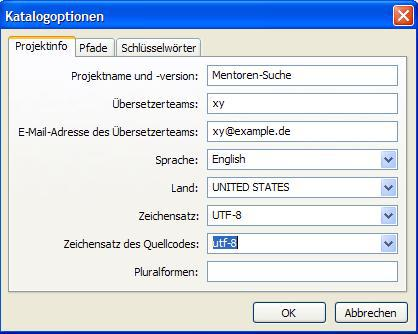
\includegraphics[angle={360}, scale=0.45]{pictures/lok1.jpg}
	    \caption{Katalogoptionen - Reiter ,,Projektinfo''}
	    \label{img:KRP}
	\end{center}
   \end{figure}
   \item \emph{Reiter „Pfade“}: Hier wird der relative Pfad, ausgehend vom Plugin-Sprachverzeichnis zum  Plugin-Basisverzeichnis angegeben. Zur Erinnerung: in diesem Beispiel nannte sich das Sprachverzeichnis „lang“, dass direkt im Plugin-Basisverzeichnis liegt. 
   \item Als Pfad muss hier also eingegeben werden: „..“ (2 Punkte für das Wechseln in eine Verzeichnisebene nach oben) (vgl. Abbildung \ref{img:KRPF}).
   \begin{figure}[htbp]
	\begin{center}
	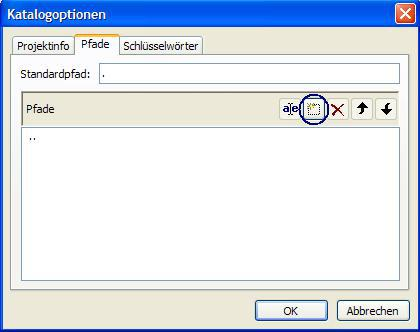
\includegraphics[angle={360}, scale=0.45]{pictures/lok2.jpg}
	    \caption{Katalogoptionen - Reiter ,,Pfade''}
	    \label{img:KRPF}
	\end{center}
   \end{figure}
\newpage
\item \emph{Reiter ''Schlüsselwörter''}: Hier werden die Funktionsnamen der Liste hinzugefügt, an denen die zu übersetzenden Begriffe/Phrasen erkannt werden. Das wären hier in diesem Fall: \_ \_ und \_e.  Alle bereits vorhandenen Funktionsnamen müssen aus der Liste entfernt werden (vgl. Abbildung \ref{img:KRSCH}).
   \begin{figure}[htbp]
	\begin{center}
	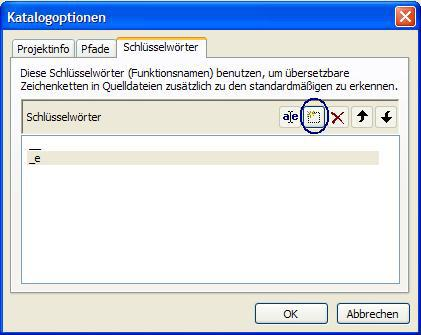
\includegraphics[angle={360}, scale=0.45]{pictures/lok3.jpg}
	    \caption{Katalogoptionen - Reiter ,,Schlüsselwörter''}
	    \label{img:KRSCH}
	\end{center}
   \end{figure}
   \item Nach Berücksichtigung aller Reiter, darf nun die Schaltfläche ''OK'' angeklickt werden. Es erscheint der Dialog ,,Speichern unter''. Die Datei sollte den Namen des Plugin-Ordners (hier: mentoren-suche) im  .pot-Format – innerhalb des Sprachverzeichnisses - abgespeichert werden. Also: mentoren-suche.pot (Anmerkung: Die \gls{POT}-Datei enthält alle Übersetzungen). Anschließend den Speichervorgang ausführen, indem die Schaltfläche ,,Speichern'' betätigt wird (vgl. Abbildung \ref{img:DSU}).
      \begin{figure}[htbp]
	\begin{center}
	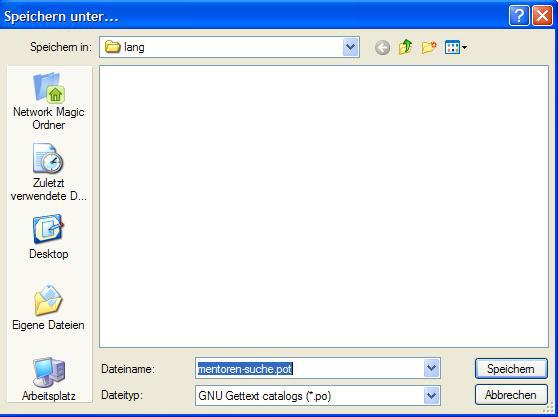
\includegraphics[angle={360}, scale=0.45]{pictures/lok4.jpg}
	    \caption{Katalogoptionen - Dialog ''Speichern unter''}
	    \label{img:DSU}
	\end{center}
   \end{figure}
   \item Nun werden alle Zeichenketten aus dem Quellcode herausgefiltert. Dazu erscheint die in der Abbildung  \ref{img:KMEUEAK} dargestellte Meldung.
     \begin{figure}[htbp]
	\begin{center}
	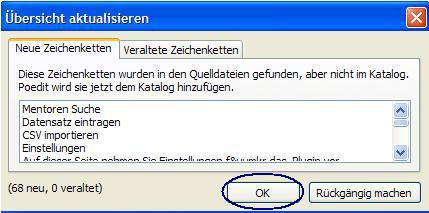
\includegraphics[angle={360}, scale=0.61]{pictures/lok5.jpg}
	    \caption{Katalogoptionen - Meldung ''Übersicht aktualisieren''}
	    \label{img:KMEUEAK}
	\end{center}
   \end{figure}   
   \newpage
   \item Nachdem Betätigen der Schaltfläche ''OK'', erscheinen alle zu übersetzenden Zeichenketten in der Oberfläche von ''Poedit'' (vgl. Abbildung \ref{img:POUEERS}).
Nun erfolgt die Übersetzung wie folgt: es wird sukzessive jede Zeichenkette vom Anwender (''Übersetzer'') angeklickt. Daraufhin erscheint im ersten unteren Textfeld die aktuelle, ausgewählte Originalzeichenkette. Im darunter liegenden Textfeld wird die entsprechende Übersetzung eingegeben. Danach wird auf das Icon ''Katalog speichern'' angeklickt. Nun ist die nächste Zeichenkette zu übersetzen. Die übersetzten Zeichenketten werden nach unten angehängt. Dies erfolgt gewöhnlich solange, bis alle Zeichenketten übersetzt sind.
     \begin{figure}[htbp]
	\begin{center}
	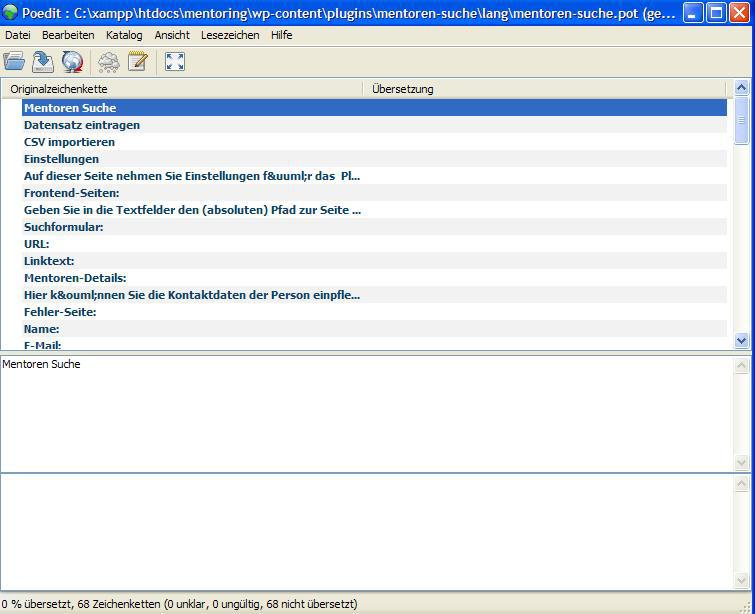
\includegraphics[angle={360}, scale=0.45]{pictures/lok6.jpg}
	    \caption{Poedit - Übersetzungen erstellen}
	    \label{img:POUEERS}
	\end{center}
   \end{figure} 
   \item Sind alle Zeichenketten übersetzt, muss eine Kopie der POT-Datei als PO-Datei
abgespeichert werden. Dies geschieht über ''Datei''  ''Speichern unter''.
Der Dateiname hat dabei folgende Konvention: \emph{pluginname-sprachcode\_Landcode.po}.
\begin{enumerate}
\item Der \emph{Sprachcode} entspricht dem Code nach ISO 639-1: siehe beispielsweise \url{http://en.wikipedia.org/wiki/List\_of\_ISO\_639-1\_codes}.
\item Der \emph{Ländercode} entspricht dem Code nach ISO 3166-1: siehe beispielsweise
\url{http://en.wikipedia.org/wiki/ISO\_3166-1}.
\end{enumerate}
Für die in diesem Beispiel englische Übersetzung (Land: USA), entsteht folgender Dateiname: \emph{mentoren-suche-en\_US.po}. 
\end{itemize}
\end{enumerate}
Damit ist der Übersetzungsprozess abgeschlossen. Es ist darauf hinzuweisen, dass neben den .po- und .pot-Dateien auch eine .mo-Datei angelegt wird. Dabei handelt es sich um eine binäre Version der .po-Datei. Diese ist nicht menschenlesbar.\footcitetgedr[Vgl.][Seite 249]{BB11}\newline
Der Prozess der Aktualisierung von bereits bestehenden Sprachdateien, soll hier nicht betrachtet werden, da dies den Rahmen dieses Tutorials sprengen würde. Denn dieser Vorgang wurde für die Entwicklung des Plugins ''Mentoren-Suche'' bisher nicht benötigt. Stattdessen wird auf Literatur Bondari/Griffiths\footcitetgedr[Vgl.][Seite 251]{BB11} verwiesen.\newline
Damit das Ergebnis der Übersetzung sichtbar ist, muss Wordpress auf die entsprechende Sprache eingestellt sein. Dies wird im nächsten Abschnitt \ref{sub:confdwpspr} beschrieben.
\subsection{Konfiguration der Wordpress-Sprache}\label{sub:confdwpspr}
Im Kapitel \ref{allgemeinesil} wurde bereits erwähnt, dass die Sprachkonfiguration von Wordpress zentral in der Konfigurationsdatei wp-config.php geschieht. In diesem Abschnitt soll vorgestellt werden, wie diese Einstellung vorgenommen wird.\newline
Die entscheidende Code-Zeile in der wp-config.php-Datei ist folgende (vgl. Listing \ref{WPLANG}).
\lstset{language={PHP},caption={wp-config.php – Die in PHP definierte Konstante WPLANG},label=WPLANG}
\lstset{
 morekeywords={function,do_action,global,\$exit_msg,\$wpdb}
}
\begin{lstlisting}
<?php 
...
define('WPLANG', 'de_DE');
...
?> 
\end{lstlisting}	
In Listing \ref{WPLANG} ist die definierte Konstante WPLANG für die zentrale Spracheinstellung der Wordpress-Oberfläche zu sehen. Der Wert der Konstante (hier: de\_DE) entspricht demselben Schema (Sprachcode/Ländercode nach ISO), wie es im Abschnitt \ref{sub:adue} beschrieben wird.\newline
Dabei ist zu beachten, dass sowohl für die jeweiligen Plugins die entsprechende Sprachdateien mitgeliefert werden müssen als auch im Wordpress-Verzeichnis wp-content/languages die Sprachdateien vorhanden sind. Ansonsten würde die Spracheinstellung keine oder nur unbefriedigende Auswirkungen haben.\newline
Zum Abschluss soll gezeigt werden, wie die Übersetzung anhand des Beispiel-Plugins ''Mentoren-Suche'' aussieht. Dazu muss in der wp-config.php (wie in diesem Abschnitt beschrieben) die Sprache englisch (für das Land USA) eingestellt werden. Der Wert für die Konstante lautet wie folgt: en\_US (kann von den Sprachdateien abgeschaut werden. Zum Beispiel:  mentoren-suche-en\_US.po).\newline
Das Ergebnis der Übersetzung wird im Folgenden für die Suchmaske im Frontend demonstriert (vgl. Abbildung \ref{img:DSDE} für die deutsche Spracheinstellung [Standard] und vgl. Abbildung \ref{img:ESEIN} für die englische Spracheinstellung).
   \begin{figure}[htbp]
	\begin{center}
		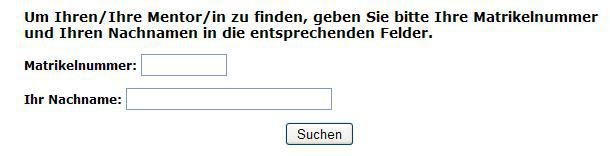
\includegraphics[angle={360}, scale=0.61]{pictures/de1.jpg}
	    \caption{Deutsche Spracheinstellung (de\_DE) [Standard]}
	    \label{img:DSDE}
	    	\end{center}
	    	\begin{center}
		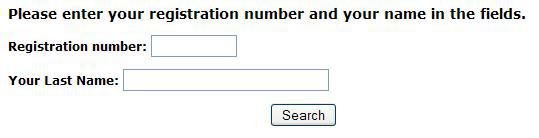
\includegraphics[angle={360}, scale=0.61]{pictures/de2.jpg}
	    \caption{Englische Spracheinstellung (en\_US)}
	    \label{img:ESEIN}
	    	\end{center}
   \end{figure} 
\ \newline
\newpage